%!TEX root = ../physical-olympics-2.tex
\chapter{光学仪器}


我们暂时不讨论光的干涉与衍射, 故暂时不太需要光的波动理论. 但实际上到了实用的层面上, 各个光学仪器, 从原理上说尽管几乎只用到几何光学的内容, 似乎也是避不开对光的强度的讨论的. 故本章先对在光的波动学说成型之前就已经蓬勃发展起来的\emph{光度学}(photometry)进行说明. 然后从若干方面对实用度最高的一些光学仪器做未免以偏概全的介绍.



\section{光度学}


光源产生的光, 在光学系统中可能被光学仪器最终接收, 如\emph{光电二极管}(photodiode), \emph{电荷耦合元件}(charge-coupled device, CCD)等. 也可以直接被人眼所直接观察. 很明显, 不同仪器作为探测仪器用时, 其光谱响应将存在很大的区别. 然而, 既然是光学, 从古到今仪器的设计都是围绕人的视觉展开. 即最核心的波段是可见光波段. 只是, 随着科技的发展, 眼睛的作用逐渐被物理仪器所替代, 对光的探测也逐渐融入了更大范围的对电磁辐射的探测中, 后者即\emph{辐射度量学}(radiometry). 比如当今天体物理中用到的各种探测手段, 从波长最长的关于宇宙微波背景的射电探测, 到波长最短的中子星$\gamma$射线暴的探测, 俨然不再是古人仰观星空可以达到的广度和深度. 辐射度量学以能量作为最基本的物理量进行测量, 单位就是焦耳, $\mathrm{J}$. 但是如果是考虑日常生活中以人眼视觉为核心设计的各类照明, 媒体灯光, 红外线, 紫外线以外的波段几乎就被我们排除在外. 为了将辐射度量学过渡到光度学我们需要先对人眼的独特的色视觉做一个了解:

\subsection{色度学*}
\begin{wrapfigure}[12]{o}[-10pt]{8cm}
\vspace{-0.4cm}
\centering
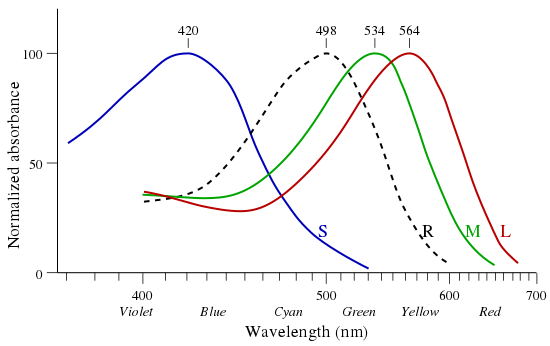
\includegraphics[width=8cm]{image/5-8-1.png}
\caption{四钟感光细胞约化吸收率}\label{fig:phtsens}
\end{wrapfigure}
大部分人类的视网膜内有两种大类的视觉感受细胞\footnote{还有\emph{内在光敏视网膜神经节细胞}(intrinsically photosensitive retinal ganglion cells, ipRGCs), 它含有\emph{视黑素}(melanopsin), 无法造成成像视觉, 但是在调节人昼夜节律方面发挥了主要功能.}:\,\emph{视锥细胞}(cone)与\emph{视杆细胞}(rod). 而视锥细胞又根据其所含视蛋白质分为感受$500-700\mathrm{nm}$波长的\emph{视红素}细胞(erythrolabe, L, $\rho$);\,感受$450-630\mathrm{nm}$波长的\emph{视绿素}细胞(chlorolabe, M, $\gamma$)和感受$400-500\mathrm{nm}$波长的\emph{视蓝素}细胞(cyanolabe, S, $\beta$)\footnote{在女性中常见异常X染色体导致个体产生四种色素的视锥细胞从而其色视觉明显优于一般的男性或女性}. 而视杆细胞由于结构差异导致比视锥细胞敏感约100倍, 单光子即可激发其\emph{视紫素}(rhodopsin, R)使其产生信号. 视紫素的合成需要依赖维生素A. 而维生素A的摄取除了动物性食物源还可以来自植物性植物中含有的$\beta$-胡萝卜素.

四种感光细胞对不同波长的光响应强度\ref{fig:phtsens}是不一致的. \emph{亮视觉}(photopic vision)才具有真正意义上的色视觉: 此时三种色素细胞L, M, S同时工作分管长, 中, 短波段的信号激励. 使得在可见光范围内的不同类似的光对三种色素细胞给出不同的激励值. 影响人对色彩的判断. 而在\emph{暗视觉}(scotopic vision)下前三种细胞失效, 视杆细胞积极发挥功能, 其视紫素R在$450-550\mathrm{nm}$波长范围有较强的吸收, 但是无法鉴别光的颜色. 所以暗视觉给人感觉接近灰度图, 同时红色物体在黑暗环境下比其它颜色物体更加昏暗. 这被称作\emph{浦金野现象}(Purkinje effect). 而有月光或星光的夜晚, 黎明与黄昏, 其实光线并没有暗到足够使得亮视觉失效. 此时的视觉称作\emph{中间视觉}(mesopic vision).

\begin{figure}[H]
\centering
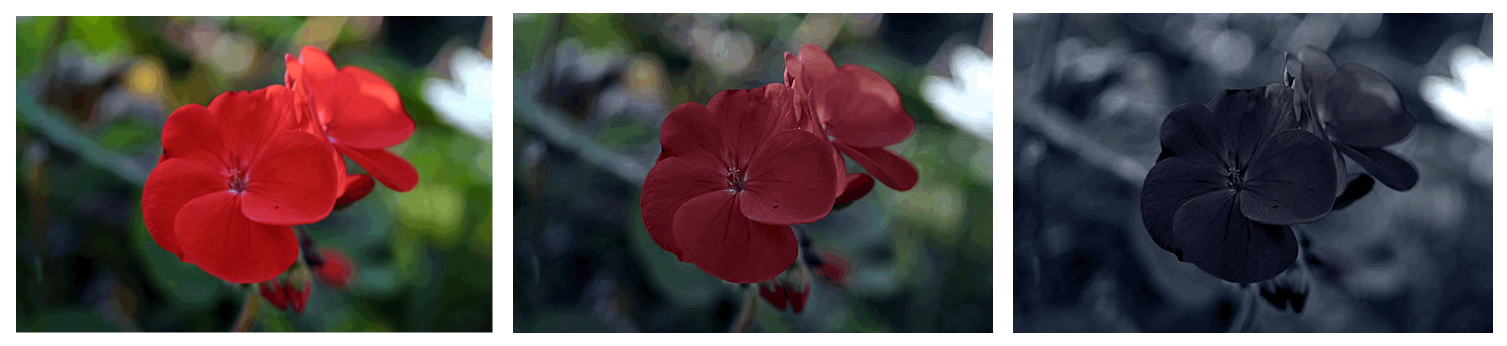
\includegraphics[width=16cm]{image/5-8-2.png}
\caption{浦金野现象}
\end{figure}

不同人的视觉条件当然存在区别. 粗的层面讲, 一束$555{\rm nm}$的位于人类视觉最敏感区的绿光和一束可见光边缘的$700{\rm nm}$的红光, 都给出$1{\rm W/m^2}$的平面波, 给人造成的亮度感觉一定是不一样的: 前者非常明亮而后者几乎不可见. 但是如果将一红一蓝两聚光灯聚焦于舞台再找两个人来比较哪个光斑更亮, 也许两个人就会给出不同的结果. 这种不同可能出于心理上或者生理上的效应. 但是如果要为照明制定标准, 就应该克服人与人之间的区别, 一般采取从大量受试者判断结果选取多数人的结果的方式. 这样就有了\emph{国际照明协会}(Commission Internationale de l\ap\'eclairage)在1931年通过的CIE1931标准. 它目前仍在广泛地被使用.

CIE1931标准将人眼中三种色素细胞的响应抽象为\emph{三激励值}(tristimulus values). 并将描述光的色彩, 亮度的空间抽象为\emph{色彩空间}(color space). 而色彩空间中的点就表示一种混合光可能的色彩与亮度, 对应三激励值L, M, S, 构成一种加性空间: 三激励值的大小代表抽象的人眼对三种抽象激励的反应. 如果以这三个参数建立坐标系表示色彩, 就称作LMS空间. 但是实用场合更常用的是另一套更直观的三激励值$XYZ$形成的空间. 它是这样定义的:

\begin{itemize}
\item $Y$定义为L, M, S的某种组合使得其恰好与混合光视觉亮度基本一致.
\item $Z$被直接定义为S值的某个倍数.
\item $X$定义为L, M, S的另一种组合使得对于所有的单色光$X$总是非负且对于可见光的矩形光谱, $X=Y=Z$.
\end{itemize}

这样经过调整就得到CIE1931标准\emph{色匹配函数}(color matching functions). 它表示不同单位能流密度的光对人眼造成的$XYZ$三激励值:

\begin{wrapfigure}[15]{o}[-10pt]{8cm}
\vspace{-0.1cm}
\centering
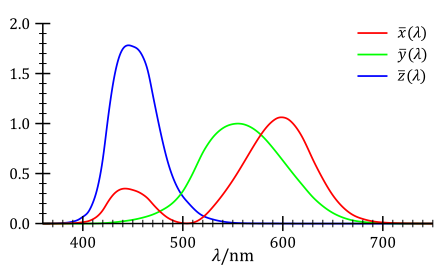
\includegraphics[width=8cm]{image/5-8-3.png}
\caption{色匹配函数}\label{fig:colormatch}
\end{wrapfigure}
直观上来看, 色匹配函数可以根据通过入射光的谱计算三激励值. 例如入射光如果总能量为$E$, 那么按照波长分解为:
\[E=\int e(\lambda)\ud \lambda\]

从而由三激励函数$\bar{x},\,\bar{y},\,\bar{z}$三激励值就是:
\[X=\int \bar{x}(\lambda)e(\lambda)\ud \lambda\]
\[Y=\int \bar{y}(\lambda)e(\lambda)\ud \lambda\]
\[Z=\int \bar{z}(\lambda)e(\lambda)\ud \lambda\]

从图中定性上可以看出$XYZ$三值的含义为: 光越亮$Y$越大, 相对$X,\,Z$值$Y$激励大则说明光中绿光成分多; 光中的蓝紫光成分越多$Z$约大; 最后$X$值越大主要说明光中的红黄光比例多, 但是实际上在$400-500{\rm nm}$的较短波长的光也能造成一定的$X$激励.

人类对色彩的理解可以分为两个大的部分: \emph{亮度}(brightness)与\emph{色度}(chromaticity). 前者为与光源亮度相匹配的关于光的整体刺激值的指标, 与三刺激值的$Y$值直接对应. 后者则是独立于亮度的纯粹描述三刺激值混合比例的性质. 而色度由于三刺激值比例接近$1:1:1$时给出特殊的色彩感受: 白色. 故确定好白点之后又可以细分为\emph{色相}(hue)和\emph{饱和度}(saturation). 饱和度为零对应的颜色即黑, 白, 灰. 随着饱和度增加, 较低饱和度的图像一般柔和, 粉润; 较高饱和度的图像则对比鲜明, 大红大绿, 视觉冲击力较强.色相则较为复杂, 可以参考下面要介绍的色度图.

为了更准确地单独描述色度. 我们引入导出的色度参数:
\[x=\frac{X}{X+Y+Z}\quad ,\quad y=\frac{Y}{X+Y+Z}\quad ,\quad z=\frac{Z}{X+Y+Z}\]

由于$x+y+z=1$, 故通常$z=1-x-y$由$x,\,y$来确定. 我们就可以用$x,\,y$来描述色度, 用$Y$来描述亮度. 尤其是, 把不同$(x,\,y)$值对应的颜色画在一个图中, 就构成了著名的\emph{色度图}(chromaticity diagram)\footnote{由于打印机颜料限制你看到的色度图边缘颜色其实已经失真了.}. 

\begin{figure}[H]
\centering
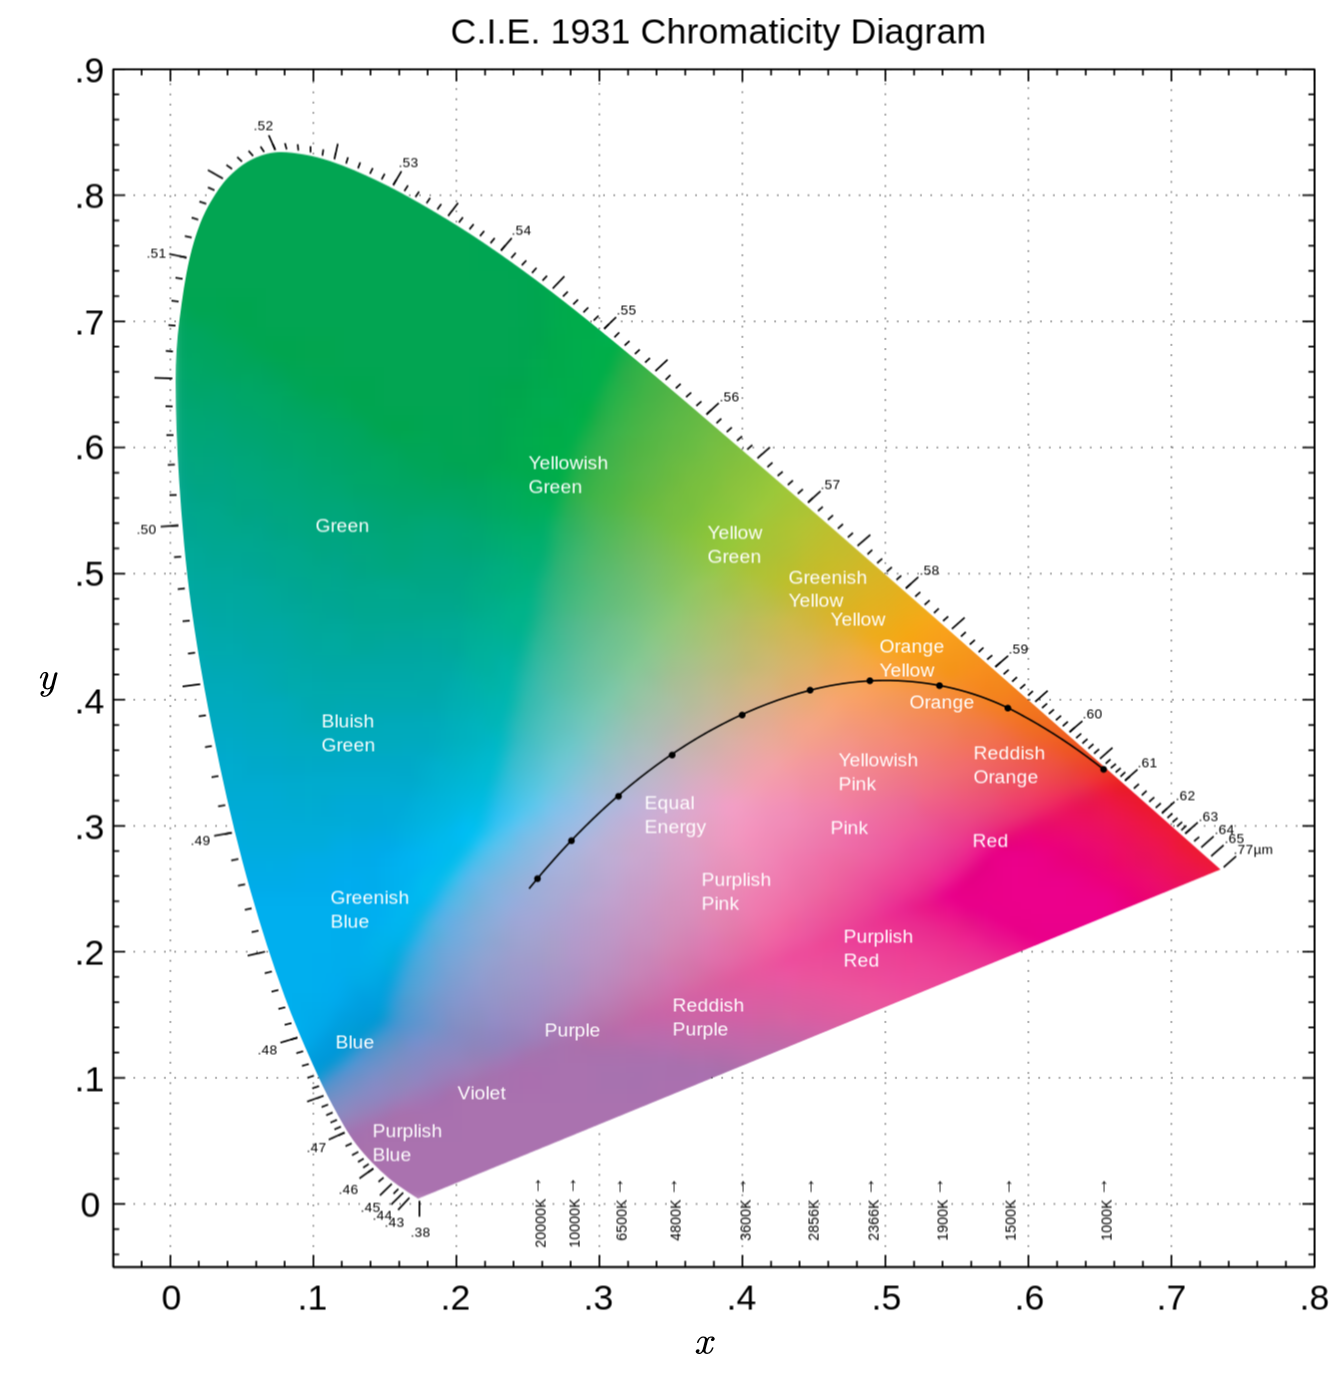
\includegraphics[width=15cm]{image/5-8-4.png}
\caption{CIE1931色度图}
\end{figure}

从色度图上可以读出:

\begin{itemize}
\item 并不是色度图上每一个点都代表实际的某种光产生的三激励值. 而是分布在一个舌形的\emph{视觉色域}(gamut of vision)中. 例如$(X,\,Y,\,Z)=(0.5,\,0.1,\,0.4)=(x,\,y,\,z)$就不是一个存在于自然界的色彩. 除非考虑生理视觉的非线性效应否则无法产生这样的三激励值, 它们对应\emph{不可能颜色}(impossible color).
\item 视觉色域被包含在由\emph{光谱色线}(spectral locus)和\emph{紫红色线}(line of purples)组成的凸轮廓内. 轮廓上就是饱和度为$1$的色彩, 它包括两类色相: 由所有单色可见光带来的色彩都在这个轮廓的曲边缘上, 即光谱色线, 色相就是我们常说的红, 橙,\,黄,\,绿,\,青,\,蓝,\,蓝紫; 由可见光边缘的红色与紫色混合形成的色彩都在这个轮廓的直边缘上, 即紫红色线, 色相包括蓝紫,\,紫,\,红紫,\,品红,\,红.
\item 光谱色线对光波长的分布绝不是均匀的. 小于$470{\rm nm}$和大于$600{\rm nm}$的紫, 红光造成的三激励值区别不大, 在色度图中压缩在较短的两端色线内. 黄绿蓝三色在色度图中具有较长的色线.
\item 一般定义\emph{白点}(white point)为矩形光谱(单位波长间隔具有相等能量$e(\lambda)={\rm const.}$)所对应的点, 按照三激励值定义它为$(x,\,y)=(1/3,\,1/3)$. 白点的饱和度定义为零.
\item 白点与边缘点的连线上所有颜色共享一个色相, 饱和度从从中心的$0$过渡到边缘的$1$.
\item 混合两种颜色的光时得到的颜色将落在色度图两颜色代表的点的连线上某点代表的颜色上.
\item 图中还标出了\emph{普朗克色线}(Planckian locus). 它们表示不同温度下黑体辐射光谱在可见光波段进行混合导致的色彩. 它历经的颜色为: 红,\,橙,\,橘黄,\,淡黄,\,白,\,淡蓝.
\end{itemize}

为了方便显示与印刷行业, 在色度图中选取\emph{原色}(primary colors)作为表示颜色的三个基, 进行混合就能产生色度图中一定范围内的色彩. 一般用的多的是\emph{RGB三色模型}(trichromatic RGB model). 在1931CIE标准中选取的三原色均来自可见光谱的红绿蓝三种单色光, 波长分别为$700{\rm nm},\,546.1{\rm nm},\,435.8{\rm nm}$, 定义其$(r,\,g,\,b)$值分别为$(1,\,0,\,0),\,(0,\,1,\,0),\,(0,\,0,\,1)$. 

\begin{wrapfigure}[15]{o}[-10pt]{7cm}
\vspace{-0.4cm}
\centering
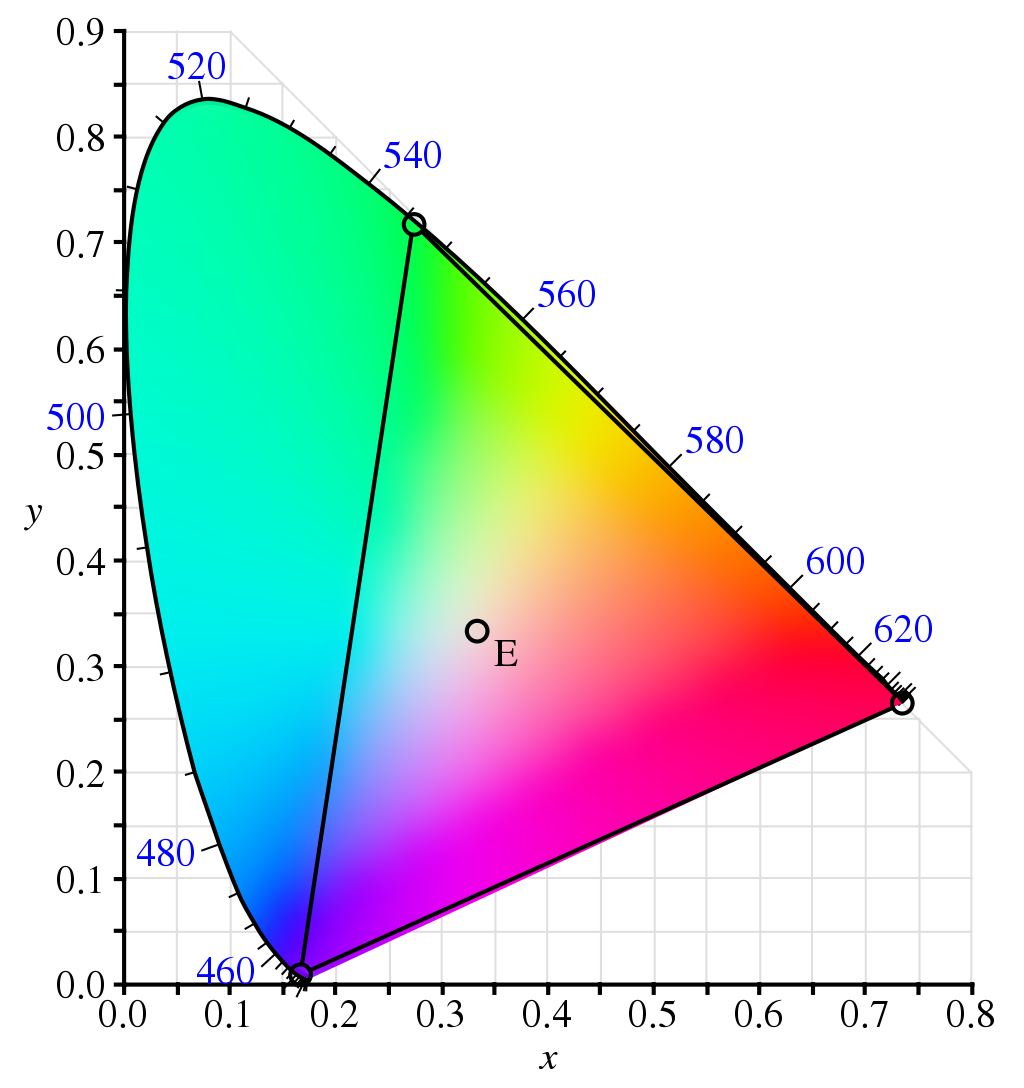
\includegraphics[width=7cm]{image/5-8-5.png}
\caption{CIE1931-RGB色域}\label{fig:rgbgamut}
\end{wrapfigure}
这实际上对应了一个线性变换:
\[{\displaystyle {\begin{bmatrix}X\\Y\\Z\end{bmatrix}}={\frac {1}{0.176\,97}}{\begin{bmatrix}0.490\,00&0.310\,00&0.200\,00\\0.176\,97&0.812\,40&0.010\,63\\0.000\,00&0.010\,00&0.990\,00\end{bmatrix}}{\begin{bmatrix}R\\G\\B\end{bmatrix}}}\]

并且$(r,\,g,\,b)$值定义为:
\[r=\frac{R}{R+G+B}\]
\[g=\frac{G}{R+G+B}\]
\[b=\frac{B}{R+G+B}\]

RGB模型将三原色进行一定比例的混合后无法覆盖色度图中的每个颜色, 而是只能产生以三原色为顶点的三角形中的色彩. 而不同行业, 乃至同一行业的不同规范使用的三原色标准点也是各不相同的. 从而也就具有不同形状的\emph{色域}(color gamut). 例如由惠普与微软与1996年提出了用于显示器, 打印机与因特网的sRGB标准就仅涵盖40\%的视觉色域面积.

CIE在1931年之后还相继公布了1964, 1976标准, 时代在进步, 关于色彩的理论和技术都在慢慢发展与变革. 后世新的标准将会逐渐取代旧标准.

\subsection{国际单位与光度函数}

对于光度学, 国际单位制有一基本单位给一个光度学物理量: \emph{发光强度}(lumious intensity). 这个基本单位为\emph{坎德拉}(candela). 众所周知, 物理量的大小总是与一定的测量过程对应, 而其单位总是与测量所采用的标准相对应. 那么以下国际单位中有关测量和其标准的规定就定义了发光强度和坎德拉两个概念:

\begin{verse}
坎德拉(cd)的定义为: 取千克, 米和秒的国际单位定义. 则频率为$540\times 10^{12}{\rm Hz}$的单色光源辐射的发光效率具有固定的数值: $683\, {\rm cd\cdot sr/W}$.
\end{verse}

这其实就是说, 如果一个频率为$540\times 10^{12}{\rm Hz}$的单色点光源向四面八方均匀发光, 辐射强度为$1{\rm W/sr}$(即具有总功率$4\pi\, {\rm W}$). 则其具有的发光强度就规定为$683{\rm cd}$. 这样任意一个同为$540{\rm THz}$, 即约$555.016{\rm nm}$的单色光源的发光强度就可以进行测量: 只需要看其辐射强度为之前的辐射强度为$1{\rm W/sr}$的光源的$x$倍, 那么相应的发光强度就是$x\cdot 683{\rm cd}$.

但是这就带来一个问题, 如何定义一个波长非$555.016{\rm nm}$的单色光源, 或是非单色光源的发光强度? 这就又重新依赖于国际单位制以外的标准, 依然以CIE1924标准为例, 它定义了一个\emph{光度函数}(luminosity function). 它可以想象为利用同为$1{\rm W/sr}$的不同波长的单色光照明对人造成的相对视觉亮度. 实验发现人在$555{\rm nm}$左右的绿光最敏感, 看上去光最亮. 故作为标准规定此时光度函数值为$1$. 其他光度函数值均相对这个标准值比较. 其值见下一页表格\ref{tab:lumtab}\footnote{此为较粗的数据表格, 更详细的数据可以参考\url{http://cvrl.ioo.ucl.ac.uk/cie.htm}}.

\begin{wrapfigure}[12]{o}[-10pt]{7cm}
\vspace{-0.4cm}
\centering
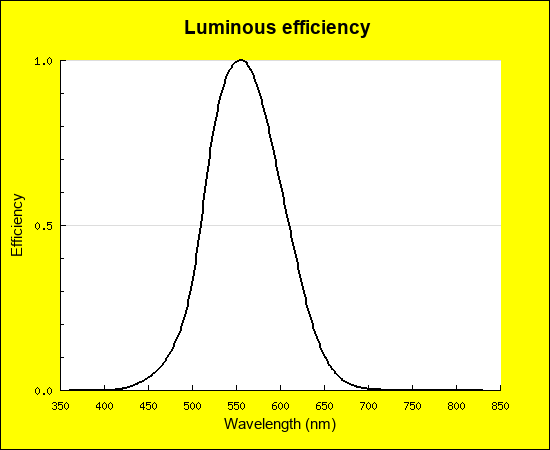
\includegraphics[width=7cm]{image/5-8-6.png}
\caption{光度函数图像}
\end{wrapfigure}
这个函数就给出了波长为$\lambda$的单色点光源辐射强度$I$与其发光强度$\mathfrak{I}$之间的换算关系, 本书用斜体罗马字母表示光度量量而哥特体字母表示原始的辐射度量量:
\[I=683.002\footnote{你没看错, 由于国际单位制(SI)与国际照明协会(CIE)标准不统一($540{\rm THz}$定标与$555{\rm nm}$定标)而是略有差距, 导致非$555{\rm nm}$的$540{\rm THz}$处光度函数小于1而需要靠略大于$683$的系数来补偿.}{\rm cd\cdot sr/W}\,\cdot V(\lambda)\cdot \mathfrak{I}\]

最后, 如果光源发光为连续谱, 那么就定义其辐射强度谱函数$\mathfrak{i}(\lambda)$:
\[\mathfrak{I}=\int \mathfrak{i}(\lambda)\ud \lambda\]

于是发光强度就为:
\[I=683.002{\rm cd\cdot sr/W}\,\cdot \int V(\lambda)\mathfrak{i}(\lambda)\ud \lambda\]

最好的方式是把辐射强度谱函数$\mathfrak{i}(\lambda)$换算为发光强度谱函数$i(\lambda)$:
\[I=\int i(\lambda)\ud \lambda\]
\[i(\lambda)=683.002{\rm cd\cdot sr/W}\,\cdot V(\lambda)\cdot \mathfrak{i}(\lambda)\]

逐渐的我们体会到, 任何描述辐射度量的物理量, 按照波长进行分解后, 乘以固定的系数$683.002$与对应波长的光度函数以后, 再对不同波长重新合成, 就构成了描述光度量的函数\footnote{这是一种广义的``点乘''或``内积'', 你体会到了吗?}. 从而有以下对应关系, 下一小节我们讲介绍关键的光度学量:

\begin{table}[H]
\centering
\caption{光度学与辐射度量学的对应}
\begin{tabular}{cc|cc}
\toprule
光度学量& 国际单位&辐射度量学量&国际单位\\
\midrule
光能量(luminous energy)&${\rm lm\cdot s\,,\, (T)}$&能量&${\rm J}$\\\midrule
光功率(luminous power)&\multirow{2}{*}{${\rm lm}$}&(辐射)功率(radiant power)&\multirow{2}{*}{${\rm W}$}\\
\cmidrule{1-1}\cmidrule{3-3}
光通量(luminous flux)& &辐射通量(radiant flux)& \\\midrule
发光强度(luminous intensity)&${\rm cd}$&辐射强度(radiant intensity)&${\rm W/sr}$\\\midrule
亮度(luminance)&${\rm cd/m^2\,,\,(nit)}$&辐射率(radiance)&${\rm W/sr\cdot m^2}$\\\midrule
照度(illuminance)&\multirow{2}{*}{${\rm lm/m^2\,,\, lx}$}&辐照度(irradiance)&\multirow{2}{*}{${\rm W/m^2}$}\\
\cmidrule{1-1}\cmidrule{3-3}
光出射度(luminous exitance)&&辐射度(radiosity)&\\
\bottomrule
\end{tabular}
\end{table}

\begin{table}[H]
\caption{光度函数表}\label{tab:lumtab}

\hfil
\begin{minipage}{0.19\textwidth}
\begin{tabular}{cc}
\toprule
$\lambda/{\rm nm}$ & $V(\lambda)$ \\
\midrule
380 & 3.90E-05 \\
385 & 6.40E-05 \\
390 & 1.20E-04 \\
395 & 2.17E-04 \\
400 & 3.96E-04 \\
405 & 6.40E-04 \\
410 & 1.21E-03 \\
415 & 2.18E-03 \\
420 & 4.00E-03 \\
425 & 7.30E-03 \\
430 & 1.16E-02 \\
435 & 1.68E-02 \\
440 & 2.30E-02 \\
445 & 2.98E-02 \\
450 & 3.80E-02 \\
\bottomrule
\end{tabular}
\end{minipage}
\begin{minipage}{0.19\textwidth}
\begin{tabular}{cc}
\toprule
$\lambda/{\rm nm}$ & $V(\lambda)$ \\
\midrule
\vdots & \vdots\\
455 & 4.80E-02 \\
460 & 6.00E-02 \\
465 & 7.39E-02 \\
470 & 9.10E-02 \\
475 & 1.13E-01 \\
480 & 1.39E-01 \\
485 & 1.69E-01 \\
490 & 2.08E-01 \\
495 & 2.59E-01 \\
500 & 3.23E-01 \\
505 & 4.07E-01 \\
510 & 5.03E-01 \\
515 & 6.08E-01 \\
520 & 7.10E-01 \\
\bottomrule
\end{tabular}
\end{minipage}
\begin{minipage}{0.19\textwidth}
\begin{tabular}{cc}
\toprule
$\lambda/{\rm nm}$ & $V(\lambda)$ \\
\midrule
\vdots & \vdots\\
525 & 7.93E-01 \\
530 & 8.62E-01 \\
535 & 9.15E-01 \\
540 & 9.54E-01 \\
545 & 9.80E-01 \\
550 & 9.95E-01 \\
555 & 1 \\
560 & 9.95E-01 \\
565 & 9.79E-01 \\
570 & 9.52E-01 \\
575 & 9.15E-01 \\
580 & 8.70E-01 \\
585 & 8.16E-01 \\
590 & 7.57E-01 \\
\bottomrule
\end{tabular}
\end{minipage} 
\begin{minipage}{0.19\textwidth}
\begin{tabular}{cc}
\toprule
$\lambda/{\rm nm}$ & $V(\lambda)$ \\
\midrule
\vdots & \vdots\\
595 & 6.95E-01 \\
600 & 6.31E-01 \\
605 & 5.67E-01 \\
610 & 5.03E-01 \\
615 & 4.41E-01 \\
620 & 3.81E-01 \\
625 & 3.21E-01 \\
630 & 2.65E-01 \\
635 & 2.17E-01 \\
640 & 1.75E-01 \\
645 & 1.38E-01 \\
650 & 1.07E-01 \\
655 & 8.16E-02 \\
660 & 6.10E-02 \\
\bottomrule
\end{tabular}
\end{minipage}
\begin{minipage}{0.19\textwidth}
\begin{tabular}{cc}
\toprule
$\lambda/{\rm nm}$ & $V(\lambda)$ \\
\midrule
\vdots & \vdots\\
665 & 4.46E-02 \\
670 & 3.20E-02 \\
675 & 2.32E-02 \\
680 & 1.70E-02 \\
685 & 1.19E-02 \\
690 & 8.21E-03 \\
695 & 5.72E-03 \\
700 & 4.10E-03 \\
705 & 2.93E-03 \\
710 & 2.09E-03 \\
715 & 1.48E-03 \\
720 & 1.05E-03 \\
725 & 7.40E-04 \\
730 & 5.20E-04 \\
\bottomrule
\end{tabular}
\end{minipage}
\hfil
\end{table}


\subsection{亮度与照度}

从实用主义的角度来看, 首先我们关心一个点光源单位时间发出的能量, 或者单位时间通过空间中某个指定的面的光具有的能量, 这个量就是功率或辐射通量, 两者具有共同的单位瓦特, 前者其实就是后者当面闭合且包裹光源时的情形. 与之对应的光度学物理量就是\emph{光通量}(luminous flux, lumens), 国际单位就是\emph{流明}(lumen). 记做${\rm lm}$. 它是一个实用频率非常高的单位, 从电灯发光的强度描述, 到室内照明的规范标准都可以看到它的身影. 对于$555{\rm nm}$的单色绿光, $1{\rm W}$的辐射通量就相当于约$683.002{\rm lm}$的光通量. 这个常数称为\emph{最大光视效能}(maximum lumious efficacy). 它的取值为:
\[K_m=683.002 {\rm lm/W}\]

而一个其他波长的单色光源的光视效能就会降低为$K(\lambda)=V(\lambda)\cdot K_m$. 那么如果一个光源的辐射通量谱分布为:
\[\mathfrak{P}=\int \mathfrak{p}(\lambda)\ud \lambda\]

它发出的流明数就可以这样计算得到:
\[\varPhi=\int K(\lambda)\mathfrak{p}(\lambda)\ud \lambda\]

不同波长的$K(\lambda)$以不同的大小把瓦特换算为流明. 最后光源自己的\emph{光视效能}(lumious efficacy)就被定义为:
\[K=\frac{\varPhi}{\mathfrak{P}}\]

一支一体式荧光灯(俗称日光灯)的典型数据为$23{\rm W},\,1500{\rm lm}$. 而如果使用发光二极管(LED)灯, 相同流明数的白光功率需求可以降低一半多, 即达到$200{\rm lm/W}$左右的能效系数. 黑体辐射则最高只有$95{\rm lm/W}$左右的能效系数, 在黑体温度约$6500{\rm K}$时达到极限.

点光源向不同方向发光的情况不一定是均匀的. 为了描述不同方向的发光强度引入单位立体角内的光通量, 即\emph{发光强度}(luminous intensity):
\[I=\frac{\ud\varPhi }{\ud \Omega}\]

电子行业的发展使得面光源发光成为照明的主要情形, 任何电子产品的显示界面就是一个面光源. 而我们也关心一个面受到照射的强度情况. 从而就产生了照度和亮度两个新的概念.

\emph{照度}(illuminance)描述被照射面单位面积从四面八方被照射的总光通量:
\[E=\frac{\ud \varPhi}{\ud S}\]

\emph{亮度}(luminance)则更为复杂, 它本应是面光源单位面积朝某特定方向的发光强度. 但是若该方向与发光面法向夹角为$\theta$, 则定义变为:
\[B=\frac{\ud I}{\ud S\cos\theta}=\frac{\ud\varPhi }{\ud \Omega\ud S\cos\theta}\]

这是因为, 如果一个发光面元朝四边八方的单位立体角内发光强度正比于该方向与发光面法向夹角的余弦$\cos\theta$, 这种余弦发光体称为\emph{朗伯体}(Lambertian body), 它就具有特殊的研究价值: 比如黑体辐射与漫反射都遵从这种发光性质. 从而把这种发光定义为各个方向亮度一致的, 注意到上式中$\ud S\cos\theta=\ud S_{\perp}$, 故朗伯体的发光面积即发光方向看过去的投影面积. 用来算亮度时的面积也用的是这个面积.

\subsection{光度学守恒量}

\begin{itemize}
\item \emph{光扩展量}(etendue)守恒: 
\[\ud G=n^2 \ud S \cos\theta \ud \varOmega\]
\item \emph{拉格朗日-亥姆霍兹不变性}(Lagrange-Helmholtz invariance): 
\[nyu=n'y'u'\]
\item 亮度不变性: 
\[B=B'\]
\end{itemize}


\section{光阑与光瞳}

\subsection{光阑}

\begin{itemize}
\item \emph{光阑}(stop)定义: 阻碍光传播的客观对象(如光圈, 透镜边缘, 镜筒等).
\item \emph{孔径光阑}(aperture stop): 起到限制最后像的范围或人能观察到的像的范围的作用. 缩小非孔径光阑的视场光阑能改变像的面积, 不改变像的照度.
\item \emph{视场光阑}(field stop): 起到限制系统能通过的光的夹角大小的作用. 缩小非视场光阑的孔径光阑能改变像的照度, 不改变像的面积.
\end{itemize}

\subsection{光瞳}

\begin{itemize}
\item \emph{光瞳}(pupil)定义: 光阑本身或光阑经过成像系统成的像.
\item \emph{入射光瞳}(entrance pupil): 物镜方的光瞳. 最好与物镜孔径匹配.
\item \emph{出射光瞳}(exit pupil): 目镜方的光瞳. 最好与人眼瞳孔直径匹配.
\end{itemize}

\section{常见仪器简介}

\subsection{人眼}

\begin{itemize}
\item 人眼明视距离 $s = 25{\rm cm}$
\item 最小分辨角 $1'$
\item 瞳孔直径 $D = 5{\rm mm}$
\item 水平视场角 $160\deg$ 竖直视场角 $130\deg$
\item 如果一个助视光学仪器是为人眼设计, 那么要考虑三个角度量是否合适: 视角放大率, 最小分辨角与视场角.
\end{itemize}

\subsection{显微镜}

\begin{itemize}
%\item 分类:
\item 放大镜放大率公式:
\[M=\frac{s}{f}\]
\item 光学显微镜放大率公式:
\[M=\frac{s\Delta}{f_Of_E}\]
\end{itemize}

\subsection{望远镜}

\begin{itemize}
\item 分类: 开普勒式, 伽利略式, 格里高利式, 卡塞格林式, 牛顿式\ldots
\item 开普勒望远镜放大率公式:
\[M=\frac{f_O}{f_E}\]
\end{itemize}

%\subsection{照相机}